
\documentclass{article}

\usepackage{amsfonts, amsmath, graphicx, tikz}

\begin{document}

\section{Potential results for publication}

\subsection{From an OR perspective}

Prove analytically that:
\begin{enumerate}
    \item Pitcher follows a threshold strategy in lead length. 
    \item Lead length is increasing in pickoff count. 
    \item Runs monontonic in components of state. 
\end{enumerate}

\subsection{From a baseball perspective}

Target journal: Journal of Sports Economics

\subsubsection*{Desired Results}

\begin{enumerate}
    \item What is the optimal lead distance based on current pitcher behavior? What is the corresponding run expectation?
    \item How does runner lead distance behavior differ from what would be optimal based on current pitcher behavior? How many runs are they leaving on the table?
    \item How does pitcher pickoff behavior differ from what would be optimal based on current runner behavior? How many runs are they leaving on the table?
    \item What is the optimal lead distance in the Nash equilibrium (assuming pitchers and runners behave optimally)? What is the corresponding run expectation?
    \item What would be a rule of thumb for how much you should extend your lead as the number of remaining pickoff attempts decreases? How does this interplay with count? What if you are a fast runner ($>$ 90th percentile)? Average runner? Slow runner?
\end{enumerate}

\subsubsection*{Necessary Steps}

{\bf Run game probability model.} Using 2023 data, we need to estimate regression models for the probabilities for (a) a pickoff attempt, (b) a stolen base attempt, and (c) a successful stolen base, given count, lead distance, pickoffs remaining and catcher arm strength (possibly a random effect for pitcher).\\
~\\
{\bf State space model.} We need a Markov model for the progression of an inning. {\it Note: Kritin and Mallesh shared a draft of this in August.}\\
~\\
{\bf Game solver.} Once we have the state space model and the estimated transition probabilities, we use either dynamic programming or value iteration to find the optimal policies.\\


  \section{Problem Statement}

  There is a runner on first base (second and third are empty) with no outs. The runner chooses their lead distance $d$ from first base. Knowing $d$, the pitcher decides whether to attempt a pickoff or to throw a pitch. The runner's objective is to maximize $E[R]$, the expected number of runs scored for the rest of the inning. The pitcher's objective is to minimize $E[R]$. The number of balls in the count is $b$; the number of strikes in the count is $s$; and the number of pickoffs already attempted is $p$. Once $p$ reaches 3, if the runner has not been tagged out on a pickoff attempt, they go to second base for free. The question is: How should the runner choose their lead distance $d$ (as a function of $b$, $s$, and $p$), to maximize $E[R]$?

  We can make two different assumptions about the pitcher's decision whether to attempt a pickoff. Both assumptions lead to worthwhile interpretations.
  \begin{enumerate}
      \item The decision is deterministic. Each choice yields a different run expectation, and the pitcher makes the choice to minimize run expectation.
      \item The decision is probabilistic (and we model it with data).
  \end{enumerate}

  \section{Transition Model}

  \includegraphics[width = \textwidth]{figures/flowchart.png}
  Note (SP): I think we want to expand the start state to include $p$.

\section{``Formal Model'' (Kritin)}
\section{New Model}
N = $<1,2>$, where 1 = baseman, 2 = pitcher \\\\
H = $<l, b, s, p, o, r>$ \\ \\
$l$ = $\{0, 1\}^3$ represents which bases are occupied by runners\\
$b$ = ball count \\
$s$ = strike count \\
$p$ = pickoff count \\
$o$ = out count \\
$r$ = runs scored in the inning \\\\
Z, the set of terminal states, $\subseteq$ H: \\
$\forall$ $t$ $\in$ Z, $o$ = 3. \\\\
P $\forall$ H $\setminus$ Z: P($\emptyset$) = 1 (?),\\P(h) = 2 (pitcher choosing to pickoff or pitch), $\forall$ h $\neq$ $\emptyset$\\\\
Preference Relation: 
$\forall$ $t \in Z$, $t \succ_2$ \\
Let $r_1$ and $r_2$ signify the runs scored in terminal states $t_1$ and $t_2$, respectively. Let $r_1$ $\geq$ $r_2$. Given $t_1$ and $t_2$, $t_2$ $\succ_2$ 

\section{Subgame}
$\Gamma$ = $<$ N, H$|_h$, P$|_h$, ($\succeq_i$) $>$ \\\\
N = $<1,2>$, 1 = baseman, 2 = pitcher \\\\
H$|_h$ = $< \{1,0,0,0\}, b, s, p, o, r >$, $\forall$ $b,s,p,o$ \\\\
Z$|_h$, the set of terminal states, $\subseteq$ H$|_h$: \\
$\forall$ $t$ $\in$ Z$|_h$, $o$ = 3 $\lor$ p = 2 \\\\
P$|_h$ $\forall$ H$|_h$ $\setminus$ Z$|_h$: \\
P$|_h$($\emptyset$) = 1 (baseman choosing lead distance), \\P(h) = 2 (?) \\\\
Preference Relation: \\
$\forall$ $t \in Z|_h$, where $o \in t = 3$, $t \succeq_2$\\
Let $r_1$ and $r_2$ signify the runs scored in terminal states $t_1$ and $t_2$, respectively. Let $r_1$ $\geq$ $r_2$. Given $t_1$ and $t_2$, where $o \in t = 3$, $t_2$ $\succeq_2$ \\\\
$\forall$ $t \in Z|_h$, where $p \in t = 2$, $t \succeq_1$\\
Let $r_3$ and $r_4$ signify the runs scored in terminal states $t_3$ and $t_4$, respectively. Let $r_3$ $\geq$ $r_4$. Given $t_3$ and $t_4$, where $p \in t = 2$, $t_3$ $\succeq_1$ \\

\section{Proof}
Prove cutoff strategy for pitcher: \\\\
More outs are preferable to less\\
probability of out increases as lead distance increases \\
given a lead distance, there is a threshold at which the pitcher prefers an attempt to pickoff rather than pitching to the batter. \\
\subsection{Formal Assumptions (everyone) }
\begin{enumerate}
    \item Expected runs not expected wins
\end{enumerate}

  \section{Possible Solutions}

    The problem we face is that the optimal lead distance $d^*(b, s, p)$ depends on the expected value of the start state $E[R | \{1, 0, 0, 0, b, s, p\}]$ while the expected value of the start state depends on the chosen lead distance. We have discussed three possible solutions:

    \subsection{Backward Induction}
    Starting from \{1, 0, 0, 0, 3, 2, 2\}, there are four possible subsequent states:
    \begin{enumerate}
        \item {\bf \{0, 0, 0, 1\}} {\it (terminal state, value is assumed known)}
        \item {\bf \{0, 1, 0, 0\}} {\it (terminal state, value is assumed known)}
        \item {\bf \{1, 0, 0, 0, end\}} {\it (terminal state, value is assumed known)}
        \item {\bf \{1, 0, 0, 0, 3, 2, 2\}} {\it (same as starting point, happens on foul ball)}
    \end{enumerate}
    If the pitcher attempts a pickoff, $E[R]$ becomes:
    $$
      f_1(d) \equiv P(\mbox{safe}\, |\, \mbox{pickoff},\, d,\, 2) \cdot E[R\, |\, \{0, 1, 0, 0\}]~+~(1 - P(\mbox{safe}\, |\, \mbox{pickoff},\, d,\, 2)) \cdot E[R\, |\, {0, 0, 0, 1}]
    $$
    If the pitcher does not attempt a pickoff, $E[R]$ becomes:
    \begin{align*}
      f_0(d) \equiv~& P(\mbox{steal}\, |\, d,\, 3,\, 2,\, 2) \cdot P(\mbox{safe}\, |\, \mbox{steal},\, d,\, 2) \cdot E[R\, |\, \{0, 1, 0, 0\}]\\
      & + P(\mbox{steal}\, |\, d,\, 3,\, 2,\, 2) \cdot (1 - P(\mbox{safe}\, |\, \mbox{steal},\, d,\, 2)) \cdot E[R\, |\, \{0, 0, 0, 1\}]\\
      & + (1 - P(\mbox{steal}\, |\, d,\, 3,\, 2,\, 2)) \cdot P(\mbox{PA Over}\, |\, 3,\, 2) \cdot E[R\, |\, \{1, 0, 0, 0\}, \mbox{end}]\\
      & + (1 - P(\mbox{steal}\, |\, d,\, 3,\, 2,\, 2)) \cdot (1 - P(\mbox{PA Over}\, |\, 3,\, 2)) \cdot E[R\, |\, \{1, 0, 0, 0, 3, 2, 2\}]
    \end{align*}
    Between $f_1$ and $f_0$, there is only one unknown: $x = E[R\, |\, \{1, 0, 0, 0, 3, 2, 2\}]$, which is itself a function of $f_1$ and $f_0$. SP posits that we can therefore solve for $x$---but there are some details to work out here that will require more carefully chosen notation. This will involve a one-dimensional grid search over $d$.

    Once we have $E[R\, |\, \{1, 0, 0, 0, 3, 2, 2\}]$, the induction moves backward from there. For example, the state $\{1, 0, 0, 0, 3, 2, 1\}$ can transition to a terminal state, to itself, or to $\{1, 0, 0, 0, 3, 2, 2\}$, whose value (and optimal lead distance $d^*(3, 2, 2)$) was derived in the previous paragraph. Therefore, we can use the same logic to derive $E[R\, |\, \{1, 0, 0, 0, 3, 2, 1\}]$ and $d^*(3, 2, 1)$. The same is true for $\{1, 0, 0, 0, 3, 1, 2\}$ and $\{1, 0, 0, 0, 2, 2, 2\}$---each of those states can only transition to a terminal state, to itself, or to $\{1, 0, 0, 0, 3, 2, 2\}$. Once we determine the optimal lead distance and run expectancy for those three states which are one step away from $\{1, 0, 0, 0, 3, 2, 2\}$, we continue the induction backward from there.
    
    \subsection{Iterative Optimization}
    
    If $E[R\, |\, \{1, 0, 0, 0, b, s, p\}]$ is known for each $(b, s, p)$, then finding the optimal lead distance $d^*(b, s, p)$ is easy. If the lead distance $d(b, s, p)$ is known, then calculating $E[R\, |\, \{1, 0, 0, 0, b, s, p\}]$ is easy. Begin by initializing $E[R\, |\, \{1, 0, 0, 0, b, s, p\}]$ according to the observed transitions in the dataset---corresponding to runners taking their observed leads, not the optimal leads. Using these run expectancies, solve for $d^*(b, s, p)$ (this will involve a one-dimensional grid search over $d$). Iterate these two steps until convergence:
    \begin{enumerate}
        \item Solve for $d^*(b, s, p)$ given $E[R\, |\, \{1, 0, 0, 0, b, s, p\}]$.\\
        (This will be a one-dimensional grid search for each $d^*(b, s, p)$.)
        \item Calculate $E[R\, |\, \{1, 0, 0, 0, b, s, p\}]$ given $d^*(b, s, p)$.
    \end{enumerate}
    Question: Does this converge to the globally optimal $d^*(b, s, p)$?
    
    \subsection{Full Grid Search}
    Given $d(b, s, p)$, we can calculate the transition probabilities between states and therefore the expected value of each state. Under full grid search, we try a whole bunch of possible values for $d(b, s, p)$, and we choose the value which yields the highest run expectancy for $\{1, 0, 0, 0, 0, 0, 0\}$. This full grid search is a 36-dimensional grid search, which may not be feasible.

  \newpage

  \section{Old Stuff}
  
    \subsection{Notation}
  
    $b \in \{0, 1\}^3$ represents which bases are occupied by runners\\
    $o \in \{0, 1, 2\}$ is the number of outs\\
    $c \equiv (c_b, c_s) \in \{0, 1, 2, 3\} \times \{0, 1, 2\}$ is the ball-strike count\\
    $p \in \{0, 1, 2\}$ is the number of pickoffs already attempted in this plate appearance\\
    ~\\
    $f_+: \{0, 1\}^3 \rightarrow \{0, 1\}^3$ gives occupied bases if 1B runner moves to 2B\\
    \indent e.g. $f_1((1, 0, 0)) = (0, 1, 0)$\\
    ~\\
    $f_-: \{0, 1\}^3 \rightarrow \{0, 1\}^3$ gives occupied bases if 1B runner is out\\
    \indent e.g. $f_0((1, 0, 0)) = (0, 0, 0)$\\
    ~\\
    {\it
      Note: We'll restrict ourselves to situations in which 1B is occupied and 2B is empty, meaning that $b \in \{(1, 0, 0), (1, 0 1)\}$; $f_+(b) \in \{(0, 1, 0), (0, 1, 1)\}$; and $f_-(b) \in \{(0, 0, 0), (0, 0, 1)\}$.
    }\\
    ~\\
    $A$ is the event that the pitcher attempts a pickoff\\
    $B$ is the event that the runner is safe on a pickoff attempt\\
    $C$ is the event that the runner attempts a steal\\
    $D$ is the event that the runner is safe on a steal attempt
  
    \subsection{Markov chain model}
  
    Let's define the state of the game to be $(b, o, c, p)$, which allows us to model expected runs scored to end of inning. We can use empirically observed transition probabilities between states to derive the run value of each state. We'll denote this by $R(b, o, c, p)$. However, these transition probabilities will change as we optimize lead distance.
  
    \subsection{The game within the pitch}
  
    Consider first the case where $p = 2$, i.e. the pitcher has already attempted two pickoffs since the last reset. In this case, if the pitcher attempts another pickoff and fails to catch the runner, then the runner advances for free. The decision tree below shows how the choice of lead distance affects the transition probabilities out of this state. We can construct the same decision tree for $p = 0$ and $p = 1$.
  
    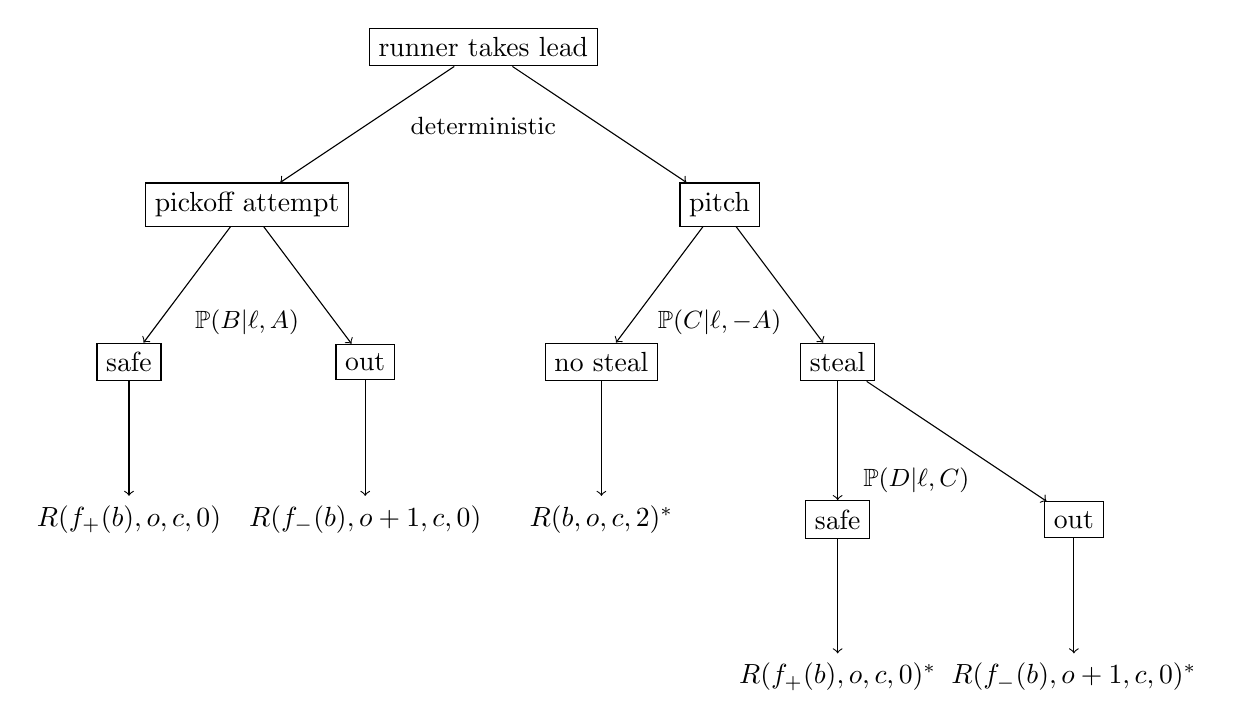
\begin{tikzpicture}[
      box/.style={draw, rectangle},
    ]
      \node[box] (1) at (4.5, 8) {runner takes lead};
      \node[box] (2) at (1.5, 6) {pickoff attempt};
      \node[box] (3) at (7.5, 6) {pitch};
      \node[box] (4) at (0, 4) {safe};
      \node[box] (5) at (3, 4) {out};
      \node[box] (6) at (6, 4) {no steal};
      \node[box] (7) at (9, 4) {steal};
      \node[box] (8) at (9, 2) {safe};
      \node[box] (9) at (12, 2) {out};
      \node (10) at (0, 2) {$R(f_+(b), o, c, 0)$};
      \node (11) at (3, 2) {$R(f_-(b), o + 1, c, 0)$};
      \node (12) at (6, 2) {$R(b, o, c, 2)^*$};
      \node (13) at (9, 0) {$R(f_+(b), o, c, 0)^*$};
      \node (14) at (12, 0) {$R(f_-(b), o + 1, c, 0)^*$};
      \node at (4.5, 7) {\small deterministic};
      \node at (1.5, 4.5) {\small $\mathbb{P}(B| \ell, A)$};
      \node at (7.5, 4.5) {\small $\mathbb{P}(C| \ell, -A)$};
      \node at (10, 2.5) {\small $\mathbb{P}(D| \ell, C)$};
      \draw[->] (1) -- (2);
      \draw[->] (1) -- (3);
      \draw[->] (2) -- (4);
      \draw[->] (2) -- (5);
      \draw[->] (3) -- (6);
      \draw[->] (3) -- (7);
      \draw[->] (7) -- (8);
      \draw[->] (7) -- (9);
      \draw[->] (4) -- (10);
      \draw[->] (5) -- (11);
      \draw[->] (6) -- (12);
      \draw[->] (8) -- (13);
      \draw[->] (9) -- (14);
    \end{tikzpicture}
    {\small
      * This isn't exactly right because the outcome state is actually a distribution over states depending on the outcome of the pitch. Hard to write down but easy to compute.
    }\\
    ~\\
    If the pitcher attempts a pickoff, the expected resulting run value is
    $$
      R_1(\ell) = \mathbb{P}(B| \ell, A) \cdot R(f_+(b), o, c, 0) + (1 - \mathbb{P}(B| \ell, A)) \cdot R(f_-(b), o + 1, c, 0).
    $$
    If the pitcher does not attempt a pickoff, the expected resulting run value is
    \begin{align*}
      R_0(\ell) = (1 & - \mathbb{P}(C| \ell, -A)) \cdot R(b, o, c, 2)^*\\
      & + \mathbb{P}(C| \ell, -A) \cdot \left(\mathbb{P}(D| \ell, C) \cdot R(f_+(b), o, c, 0)^* + (1 - \mathbb{P}(D| \ell, C)) \cdot R(f_-(b), o + 1, c, 0)^*\right)
    \end{align*}
    Logically, the pitcher should attempt the pickoff if $R_1(\ell) < R_0(\ell)$, so the runner wants to choose $\ell$ to maximize $\min\{R_0(\ell), R_1(\ell)\}$. Assuming that $\mathbb{P}(B| \ell, A)$, $\mathbb{P}(C| \ell, -A)$ and $\mathbb{P}(D| \ell, C)$ are all monotone, continuous functions of $\ell$, the optimal lead distance $\tilde \ell$ for the runner will satisfy $R_0(\tilde\ell) = R_1(\tilde\ell)$, meaning that the pitcher is indifferent to attempting a pickoff or not.
  
    However! These choice have been made to maximize $R(\cdot)$, which assumes lead distances matching empirical observation, not optimal lead distances. If the runner knows they can choose the optimal lead for the next pitch, then they want to maximize the expected runs under this optimality assumption, which we'll call $\tilde R(\cdot)$. Unfortunately, we've reached a circle in our logic, but $\tilde R(\cdot)$ would be used to calculate $\tilde \ell$, and $\tilde \ell$ would be used to calculate $\tilde R(\cdot)$.
  
    \subsection{Solving the game}
  
    I admit that I'm at a little bit of a loss here. The hack I would try is to initialize $\tilde R(\cdot)$ at $R(\cdot)$, and then alternate between using $\tilde R(\cdot)$ to calculate $\tilde \ell$ and vice versa. I imagine this will probably work well because I don't think $\tilde R(\cdot)$ will be very different from $R(\cdot)$, but I don't know whether we can guarantee convergence. Perhaps there is a way to evaluate $\tilde \ell$ and $\tilde R(\cdot)$ simultaneously, and this is what Andrew refers to as ``solving the stochastic game''?
  
    \subsection{Extensions}
  
    Right now, lead distance is the only covariate that influences baserunner advancement/elimination probabilities. But we'll also want to include information about the players involved (pitcher, catcher, runner) and additional context (count, etc.).

\end{document}